\documentclass[titlepage,12pt,a4paper,times]{book}

\usepackage[utf8]{inputenc}
\usepackage[english]{babel}
\usepackage[T1]{fontenc}
\usepackage{makeidx}
\usepackage{xspace}
\usepackage{graphicx,color,times}
\usepackage{fancyhdr}
% \usepackage{pxfonts}
% \usepackage{times}
% \usepackage{mathptm}
% \usepackage{amssymb}
% \usepackage{amsfonts}
\usepackage{amsmath}
\usepackage{latexsym}
\usepackage[printonlyused]{acronym}
\usepackage{float}
\usepackage{listings}
\usepackage{tocbibind}
\usepackage{wrapfig}
\usepackage[square]{natbib}
\usepackage{hyperref}
% \usepackage{glossaries}
% \makeglossaries
\usepackage{etoolbox}
\usepackage[section]{placeins}
\usepackage{enumitem}

% reset acronyms every chapter
\preto\chapter{\acresetall}

\renewcommand{\ttdefault}{phv}

\pagestyle{fancy}
\renewcommand{\chaptermark}[1]{\markboth{#1}{}}
\renewcommand{\sectionmark}[1]{\markright{\thesection\ #1}}
\fancyhf{} \fancyhead[LE,RO]{\bfseries\thepage}
\fancyhead[LO]{\bfseries\rightmark}
\fancyhead[RE]{\bfseries\leftmark}
\renewcommand{\headrulewidth}{0.5pt}
\renewcommand{\footrulewidth}{0pt}
\addtolength{\headheight}{0.5pt}
\setlength{\marginparsep}{0cm}
\setlength{\marginparwidth}{0cm}
\setlength{\marginparpush}{0cm}
\addtolength{\hoffset}{-1.0cm}
\addtolength{\oddsidemargin}{\evensidemargin}
\addtolength{\oddsidemargin}{0.5cm}
\addtolength{\evensidemargin}{-0.5cm}


% NEW COLORS
\definecolor{dark}{gray}{0.25}
\definecolor{lgray}{gray}{0.9}
\definecolor{dkblue}{rgb}{0,0.13,0.4}
\definecolor{dkgreen}{rgb}{0,0.6,0}
\definecolor{gray}{rgb}{0.5,0.5,0.5}
\definecolor{mauve}{rgb}{0.58,0,0.82}

\lstset{ %
  language=C,                    basicstyle=\footnotesize,
  numbers=none,                  numberstyle=\tiny\color{gray},
  stepnumber=1,                  numbersep=5pt,
  backgroundcolor=\color{white}, showspaces=false,
  showstringspaces=false,        showtabs=false,
  frame=single,                  rulecolor=\color{black},
  tabsize=2,                     captionpos=b,
  breaklines=true,               breakatwhitespace=false,
  title=\lstname,                keywordstyle=\color{blue},
  commentstyle=\color{dkgreen},  stringstyle=\color{mauve},
  escapeinside={\%*}{*)},        morekeywords={*},
  belowskip=0cm
}


\begin{document}


\thispagestyle{empty}
\setcounter{page}{-1}

\begin{center}
\begin{Huge}
\textbf{Universidade da Beira Interior}
\end{Huge}
\end{center}

\begin{center}
\begin{Huge}
Departamento de Informática
\end{Huge}
\end{center}

\vspace{0,07cm}
\begin{figure}[!htb]
\centering

\includegraphics[scale=0.3]{brasaoubi.JPG}
\end{figure}

\vspace{0.5cm}
\begin{center}
\begin{Large}
\textbf{Nº x - 2016: \emph{RTEMS}}
\end{Large}
\end{center}


\vspace{0.5cm}
\begin{center}
\begin{normalsize}
\begin{large}
Written by:
\end{large}
\end{normalsize}
\end{center}

\vspace{0.2cm}
\begin{center}
\begin{large}
\textbf{José Filipe Pereira Machado Monteiro}
\end{large}
\end{center}

\vspace{0,5cm}
\begin{center}
\begin{normalsize}
\begin{large}
Supervisor:
\end{large}
\end{normalsize}
\end{center}

\vspace{0.2cm}
\begin{center}
\begin{large}
\textbf{Prof. Dr. Paul Andrew Crocker}
\end{large}
\end{center}



\vspace{0.5cm}
\begin{center}
\begin{normalsize}
July x, 2016
\end{normalsize}
\end{center}


\clearpage{\thispagestyle{empty}\cleardoublepage}

\frontmatter
\chapter*{Acknowledgments}
\label{chap:ack}

I would like to thank very many people for putting up with me and eventually I
will write this properly, but not right now :D

\tableofcontents

\clearpage{\thispagestyle{empty}\cleardoublepage}

\listoffigures

% Se não existirem tabelas, comentar as seguintes linhas
\clearpage{\thispagestyle{empty}\cleardoublepage}

\listoftables
\clearpage{\thispagestyle{empty}\cleardoublepage}

% \listoflistings

\chapter*{Acronyms}
\begin{acronym}[SIFT]
	\acro{SVM}{Support Vector Machine}
	\acro{HOG}{Histogram of Oriented Gradient}
	\acro{BoW}{Bag of Words}
	\acro{DCT}{Discrete Cosine Transform}
	\acro{SIFT}{Scale-Invariant Feature Transform}
\end{acronym}

% \clearpage{\pagestyle{empty}\cleardoublepage}
% \chapter*{Glossary}
\makeglossaries

\newglossaryentry{.NET Framework}
{
  name={.NET Framework},
  description={É uma plataforma para desenvolvimento e funcionamento de aplicações desenvolvida pela Microsoft.}
}


\clearpage{\thispagestyle{empty}\cleardoublepage}

\mainmatter
\chapter{Introduction}
\label{chap:intro}
\nocite{*}
\section{Background}
\label{sec:amb}

\section{Motivation}
\label{sec:mot}
\section{Objectives}
\label{sec:obj}

\section{Document organization}
\label{sec:organ}
% !POR EXEMPLO!
De modo a refletir o trabalho que foi feito, este documento encontra-se
estruturado da seguinte forma:
\begin{enumerate}
\item The first chapter -- \textbf{Introduction} --
\item The second chapter -- \textbf{Other Works} --
\item The third chapter -- \textbf{Implementation} --
\item The fourth chapter -- \textbf{Results} --
\item The fifth chapter -- \textbf{Conclusions and Future Work} --
\end{enumerate}

\chapter{Other Works}
\label{chap:ow}

\section{Introduction}
\label{chap2:sec:intro}

\section{Real-Time Clothing Recognition in Surveillance Videos}
\label{chap2:sec:art1}

The video content analysis system, described in ~\citep{1}, is capable of
recognizing, in real-time, eight categories of clothing in multiple people.

As seen in the figure ~\ref{fig:vcasd} ~\citep{1}, first a face detection and
tracking are performed for each video frame. Afterwards, based on the face,
it is cropped a candidate rectangular region, containing the body of the
person. Once the face location and candidate region are known, occlusions are
conducted. These are calculated according to every face location and
overlapped areas of the rectangles. When people feature a visible frontal
face and the non-occluded area is bigger than 75\% it is possible to proceed
with clothing segmentation. The candidate rectangle region is segmented to
roughly homogeneous color segments, then applied the prior knowledge of
foreground and background, based on face alignment, in order to extract the
foreground figure. Note that, to ensure the applicability of the system it is
not utilized motion information nor background subtraction technique.

\begin{figure}[!h]
\centering
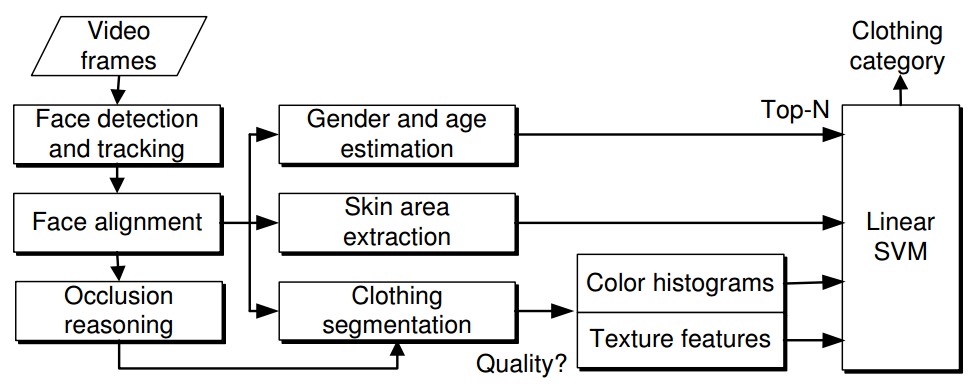
\includegraphics[scale=0.5]{images/Clothing_Diagram_1.png}
\caption{Video content analyses system diagram.}
\label{fig:vcasd}
\end{figure}
\FloatBarrier

A proper human figure alignment and clothing segmentation are required to
perform feature extraction and clothing classification. The results from
clothing segmentation might not be reliable for every frame. It is employed a
few cloth instances, with good segmentation quality, to calculate the average
feature vector to represent a cloth. A cloth is represented by ten instances,
including: gender and age estimation; skin ratio of arms and legs; 2D color
histograms; three texture descriptors.
\ac{HOG} is one of the used texture descriptors, extracting the features of
multiple spacial cells, drawn in figure ~\ref{fig:dtf}a ~\citep{1} as white
rectangles. The \ac{BoW}, another descriptor used, receives a bag of dense
\ac{SIFT} features, ~\ref{fig:dtf}b ~\citep{1}. The last texture descriptor
used is \ac{DCT}, figure ~\ref{fig:dtf}c ~\citep{1} In furtherance of better
results, clothes are analyzed in 2 sections, top and bottom, as represented
in figure ~\ref{fig:dtf} ~\citep{1}.

\begin{figure}[!h]
\centering
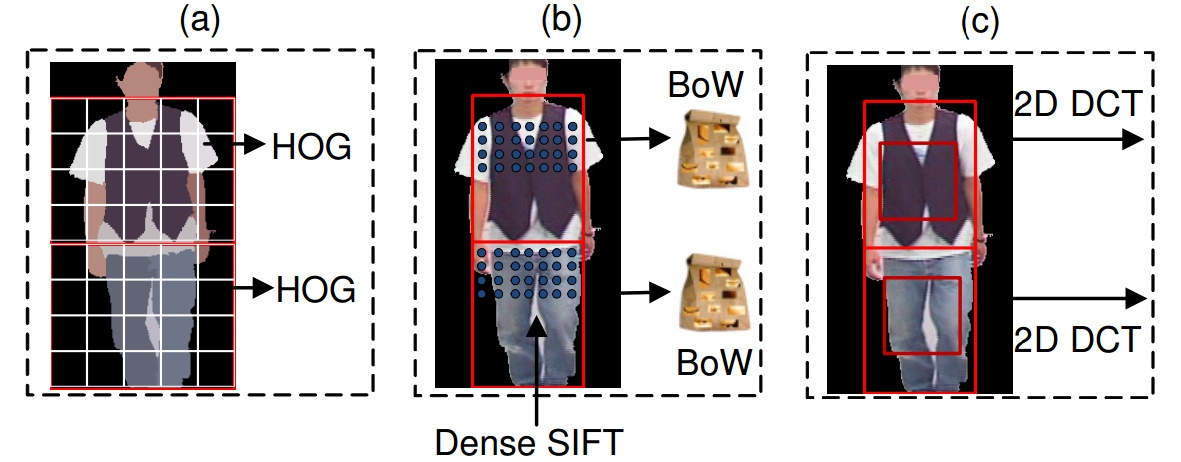
\includegraphics[scale=0.3]{images/top_bottom.jpg}
\caption{Different textures features based on \acs*{HOG}, \acs*{BoW} and
\acs*{DCT} responses.}
\label{fig:dtf}
\end{figure}
\FloatBarrier

All the previously mentioned instances of a cloth are concatenated as the
clothing representation. Each clothing category is provided to a
one-against-all linear \ac{SVM} to be learnt.

The precision rate of the presented system goes from 45.0\% up to 90.3\%,
in short-pants and short-skirts respectively, as shown in table ~\ref{tab:prds}
 ~\citep{1}.

\begin{table}
\centering
\begin{tabular}{|l|r|}
\hline
\textbf{Category} & \textbf{Precision}\\
\hline
\hline
\textbf{Suit (top)} & 87.5\% \\
\hline
\textbf{Suit (bottom)} & 85.7\% \\
\hline
\textbf{Shirt} & 81.8\% \\
\hline
\textbf{T-shirt} & 70.7\% \\
\hline
\textbf{Jeans} & 90.1\% \\
\hline
\textbf{Short pant} & 45.0\% \\
\hline
\textbf{Short skirt} & 90.3\% \\
\hline
\textbf{Long skirt} & 74.7\% \\
\hline
\end{tabular}
\caption{Precision rate of the described system.}
\label{tab:prds}
\end{table}
\FloatBarrier

\section{Describing Clothing by Semantic Attributes}
\label{chap2:sec:art2}

\section{Getting the Look: Clothing Recognition and Segmentation for Automatic
Products Suggestions in Everyday Photos}
\label{chap2:sec:art3}

\section{High-Level Clothes Description Based on Colour-Texture and Structural
Features}
\label{chap2:sec:art4}

\section{Mobile Visual Clothing Search}
\label{chap2:sec:art5}

\section{Conclusions}
\label{chap2:sec:concs}

\chapter{Implementation}
\label{chap:imp}

\section{Introduction}
\label{chap3:sec:intro}

\section{Background Subtration}
\label{chap3:sec:bs}

\section{Body Pose Estimation}
\label{chap3:sec:bps}

\section{Color and Texture Extration}
\label{chap3:sec:cte}

\section{Neural Network Training}
\label{chap3:sec:nnt}

\section{Conclusions}
\label{chap3:sec:concs}

\chapter{Results}
\label{chap:res}

\section{Introduction}
\label{chap4:sec:intro}

\section{}
\label{chap4:sec:...}

\section{Conclusions}
\label{chap4:sec:concs}

\chapter{Conclusions and Future Work}
\label{chap:cfw}

\section{Main Conclusions}
\label{sec:main-conc}

Esta secção contém a resposta à questão: \\
\emph{Quais foram as conclusões princípais a que o(a) aluno(a) chegou no fim
deste trabalho?}

\section{Future Work}
\label{sec:future-work}

Esta secção responde a questões como:\\
\emph{O que é que ficou por fazer, e porque?}\\
\emph{O que é que seria interessante fazer, mas não foi feito por não ser
exatamente o objetivo deste trabalho?}\\
\emph{Em que outros casos ou situações ou cenários -- que não foram estudados
no contexto deste projeto por não ser seu objetivo -- é que o trabalho aqui
descrito pode ter aplicações interessantes e porque?}

% SE EXISTIREM APENDICES, DESCOMENTAR O QUE ESTÁ EM BAIXO
% \appendix
% \include{apendice1}
% \clearpage{\pagestyle{empty}\cleardoublepage}
% \include{continuacao}
% \clearpage{\pagestyle{empty}\cleardoublepage}
% \include{apendice2}
% \clearpage{\pagestyle{empty}\cleardoublepage}
% \include{apendice3}
% \clearpage{\pagestyle{empty}\cleardoublepage}

\backmatter

\bibliographystyle{apalike-url}
\bibliography{bibliography}

\end{document}
